\chapter{Clustering}
In questo capitolo mostreremo il comportamento 
degli algoritmi di clustering KMeans, DBSCAN 
e Hierarchical applicati al nostro insieme di 
dati.

Il dataset utile per questa fase \`e stato
ottenuto eliminando gli attributi categorici
\texttt{education, sex} e \texttt{status} 
e l'attributo \texttt{credit\_default} 
poich\`e il clustering rientra tra 
gli addestramenti di tipo non supervisionato.

\section{KMeans}

Il miglior parametro \textit{k} con cui eseguire 
KMeans \`e stato stimato calcolando la 
\textit{SSE} variando \textit{k} su un range da 
2 a 20, con metrica di distanza euclidea. 
In figura~\ref{fig:best_k} sono riportati 
i risultati ottenuti. Si nota che il cambio di
pendenza della curva si trova quando \textit{k}
vale 7. A partire da ci\`o abbiamo eseguito l'algoritmo
per $k\in[3,10]$, reiterando per ogni passo 50 volte
KMeans per evitare che la scelta casuale dei centroidi
influenzasse i risultati e calcolando in questo caso
anche l'indice di Silhouette per i cluster trovati.
In seguito a queste analisi abbiamo constatato come
i cluster ottenuti per $k=4$ siano i pi\`u significativi,
la nostra considerazione \`e stata rafforzata dal fatto
che il clustering ottenuto per $k=4$ presenta il valore
dell'indice di \sil pi\`u alto trovato.

\begin{figure}[H]
	\centering
	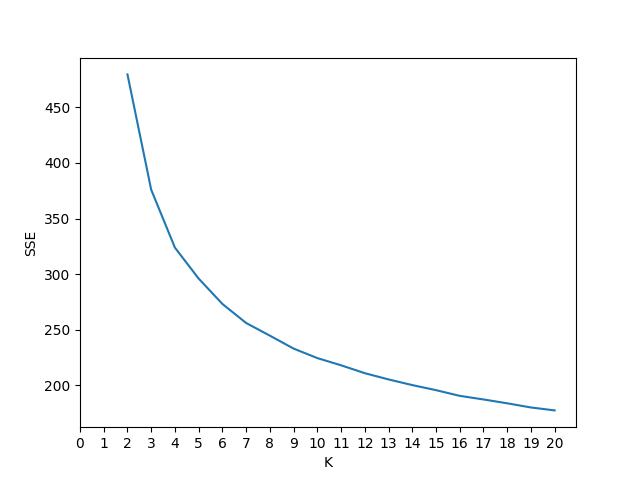
\includegraphics[width=10cm]{img/best_k.png}
	\caption[LOF entry]{SSE}
	\label{fig:best_k}
\end{figure} 

Di seguito analizziamo i cluster trovati, assegnando loro 
un nome che contraddistingua le caratteristiche 
di ogni cluster.

\paragraph{Senza rischio}
Cluster costituito da 3032 persone. Pagano in modo puntuale
le loro spese ogni mese senza registrare ritardi e compiono 
solitamente spese di bassa entit\`a. Non costituiscono alcuna
minaccia per la banca.

\paragraph{Piccoli pagatori}
Gruppo di 4832 persone. Sono soliti fare un uso abbastanza 
intensivo del revolving credit per pagare le loro spese. 
Anch'essi registrano spese di bassa entit\`a e non commettono
gravi ritardi nel pagamento, per questo motivo rientrano tra
clienti credibili per la banca.

\paragraph{Grandi pagatori}
Cluster di 1083 persone. Come per i \textit{piccoli pagatori}, 
anch'essi sono soliti usare la modalit\`a di pagamento 
rateizzata anche se le loro spese sono generalmente molto elevate.
Non si registrano comunque grossi ritardi ed \'e per questo che
rientrano comunque tra il gruppo di clienti credibili.

\paragraph{Ritardatari}
Gruppo formato da 1053 persone. Registrano spese di media entit\`a
ma al contrario degli altri tre gruppi si verificano gravi ritardi
nei pagamenti. Sono il cluster di persone che, infine, finisce in
credit default e non sono clienti credibili per la banca.

In figura~\ref{fig:centers} si sono plottate una selezione
delle coordinate dei centroidi, mostrando chiaramente dove i quattro
cluster trovati differiscono maggiormente.

\begin{figure}[H]
	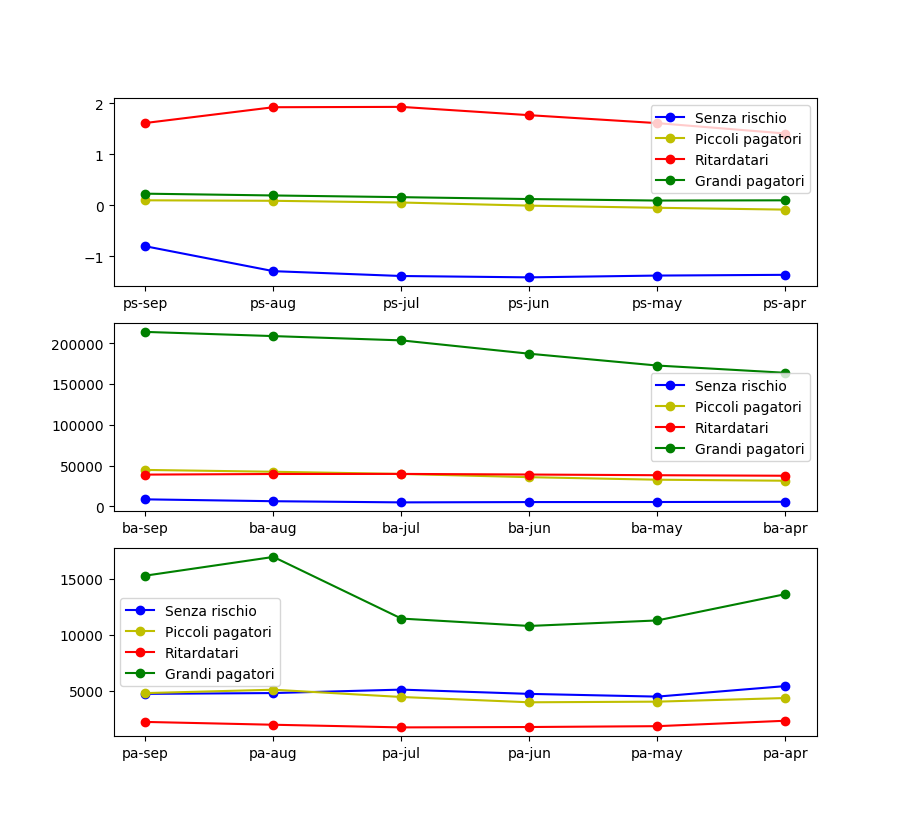
\includegraphics[width=\linewidth]{img/centers_kmeans.png}
	\caption{Caratteristiche dei cluster}
	\label{fig:centers}
\end{figure} 

\begin{figure}[H]
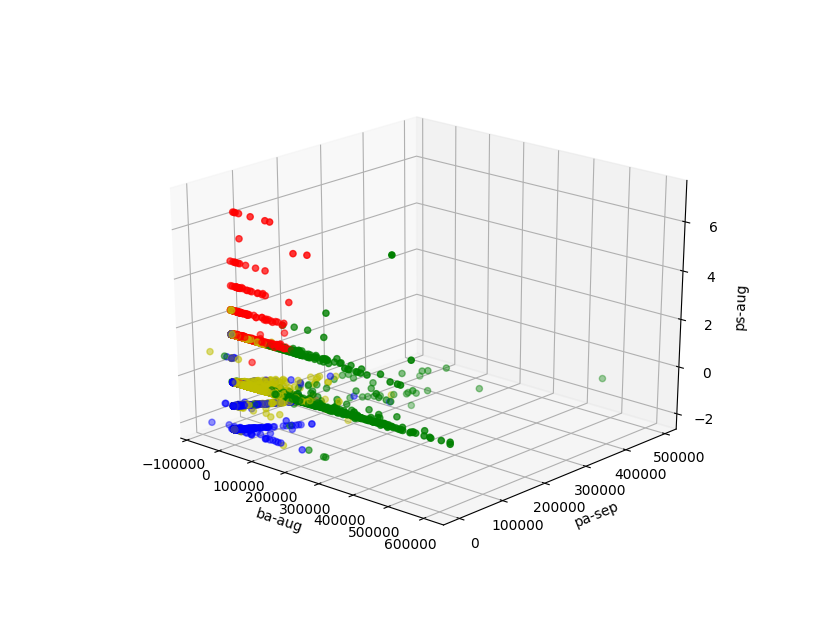
\includegraphics[width=\linewidth]{img/kmeans.png}
\caption{Distribuzione dei cluster su un pagamento mensile}
\label{fig:kmeans}
\end{figure} 

Infine si \`e plottato su un un grafico 3D (figura~\ref{fig:kmeans}
la distribuzione dei cluster su un pagamento mensile (in questo 
caso si e' preso il pagamento del mese di agosto) ed abbiamo 
notato che la distribuzione \`e rispettata per ogni terna di attributi
validi costruibili sull'insieme dei mesi disponibili.
In particolare il cluster dei \textit{ritardari} si posiziona sempre a valori molto elevati di \texttt{payment status}, mentre vale
esattamente il contrario per il cluster dei \textit{senza rischio}.
Le tre
dimensioni scelte per l'esempio sono \texttt{billing amount august},
\texttt{payment status august} e \texttt{payment amount september}.

Infine riportiamo una tabella contenente la media e la deviazione 
standard di ogni cluster individuato. Per ragioni di spazio per 
gli attributi \texttt{payment status}, \texttt{payment amount}
e \texttt{billing amount} mostriamo i valori degli ultimi due mesi.

\begin{center}
	
\begin{tabular}{c|c|c|c|c|c|c}
	\hline
	\textbf{Cluster} & \textbf{ps-sep} 
	& \textbf{ps-aug} & \textbf{pa-sep} 
	& \textbf{pa-aug}\\
	\hline
	Senza rischio & 
	$-0.8 (\pm 1.0)$ & 
	$-1.3 (\pm 0.7)$ &
	$4.7k (\pm 12.0k)$ &
	$4.8k (\pm 14.3)$\\
	\hline
	Piccoli pagatori & 
	$0.09 (\pm 0.71)$ & 
	$0.08 (\pm 0.71)$ &
	$4.8k (\pm 10k)$ &
	$5k (\pm 13.3k)$\\
	\hline
	Grandi pagatori & 
	$0.22 (\pm 0.75)$ & 
	$0.19 (\pm 0.71)$ &
	$15k (\pm 35k)$ &
	$16k (\pm 56k)$\\
	\hline
	Ritardatari & 
	$1.60 (\pm 1.18)$ & 
	$1.90 (\pm 1.03)$ &
	$2k (\pm 3.4k)$ &
	$1.8k (\pm 3.0k)$\\
	\hline
	& 
	\textbf{ba-sep} & 
	\textbf{ba-aug} & 
	\textbf{limit} & 
	\textbf{age} &\\
	\hline
	Senza rischio & 
	$8.7k (\pm 21k)$ &
	$6.4k (\pm 16k)$ &
	$215k (\pm 126k)$ &
	$36 (\pm 8)$\\
	\hline
	Piccoli pagatori &
	$44k (\pm 39k)$ &
	$42k (\pm 35k)$ &
	$130k (\pm 113k)$ &
	$35 (\pm 9)$\\
	\hline
	Grandi pagatori &
	$213k (\pm 93k)$ &
	$208k (\pm 88k)$ &
	$281k (\pm 115k)$ &
	$37 (\pm 8)$\\
	\hline
	Ritardatari &
	$38k (\pm 35k)$ &
	$39k (\pm 36k)$ &
	$79k (\pm 68k)$ &
	$34 (\pm 8)$\\
	\hline
	& 
	\textbf{sex} & 
	\textbf{status} & 
	\textbf{education} & 
	\textbf{default}\\
	\hline
	Senza rischio & 
	F &
	Single &
	University&
	17\%\\
	\hline
	Piccoli pagatori & 
	F &
	Single &
	University&
	18\%\\
	\hline
	Grandi pagatori & 
	F &
	Single &
	University&
	19\%\\
	\hline
	Ritardatari & 
	F &
	Single &
	University&
	61\%\\
	\hline
\end{tabular}

\end{center}

Si noti come il gruppo dei ritardatari ha un limite imposto dalla banca molto pi\`u basso rispetto agli altri cluster. Segno che la banca ha valutato ottimamente i profili nella scelta di concessione del credito.

\section{DBSCAN}
\newpage


\section{Hierarchical Clustering}
Per l'algoritmo di Hierarchical Clustering si è utilizzato un dataset privo delle varibili categoriche \texttt{education, status, sex} e della variabile \texttt{credit\_default}, poichè come più volte sottolineato, l'addestramento è di tipo non supervisionato. Inoltre dopo una serie di test si è deciso di eliminare anche la variabile \texttt{age}, senza la quale si sono raggiunti buoni risultati. Per parametri del clustering gerarchico si è scelta la \textbf{formula euclidea} per la distanza dato che l'utilizzo delle metriche \textit{supremum e manhattan} ha portato alla generazione di clusters di cardinalità troppo diverse. Per lo stesso motivo si è scelto come metodo aggregativo il \textbf{Metodo di Ward}, o della devianza minima, attraverso il quale si è raggiunto il miglior risultato in termini di ordine di grandezza delle dimensioni dei cluster. Gli altri metodi utilizzati $($single, complete, average$)$ non hanno portato a risultati accettabili.
\begin{figure}[H]
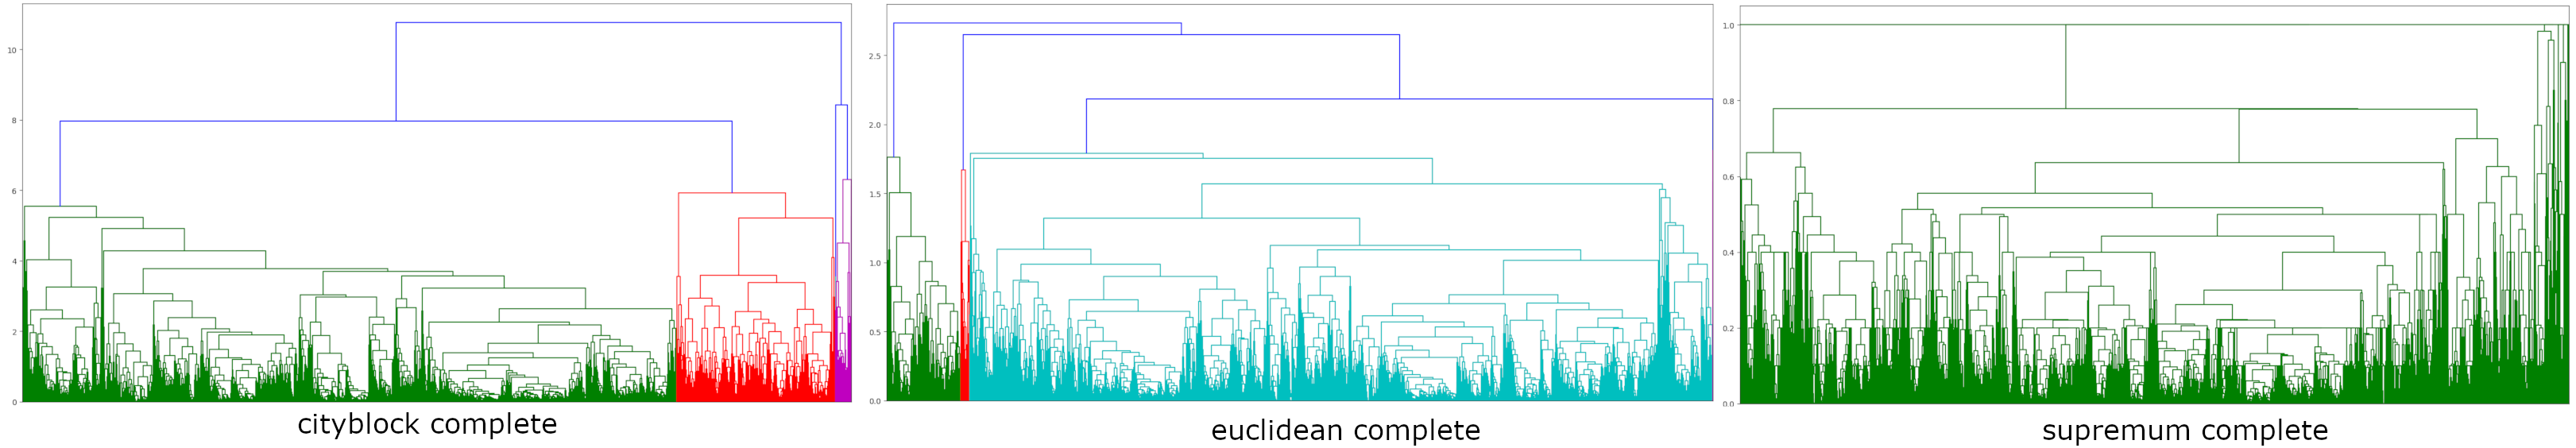
\includegraphics[width=\linewidth]{img/complete.png}
\caption{Esempio di dendrogrammi ricavati durante il test. I 3 casi in figura non sono stati considerati cluster accettabili.}
\label{dendro-complete}
\end{figure} 
\mbox{}\\
\mbox{}\\
Utilizzando la metrica euclidea e il metodo di Ward per il merging, si è deciso di settare la soglia a 15.2 ottenendo 4 cluster di dimensioni comparabili. In figura~\ref{euward} sono visualizzabili i clusters ottenuti mentre in figura ~\ref{euwardtrunc} è stato effettuato raggruppamento dei non singleton più profondi e sono stati aggiunti dei label per effettuare il troncamento a 15.2.
\begin{figure}[!htb]
\minipage{0.48\textwidth}
  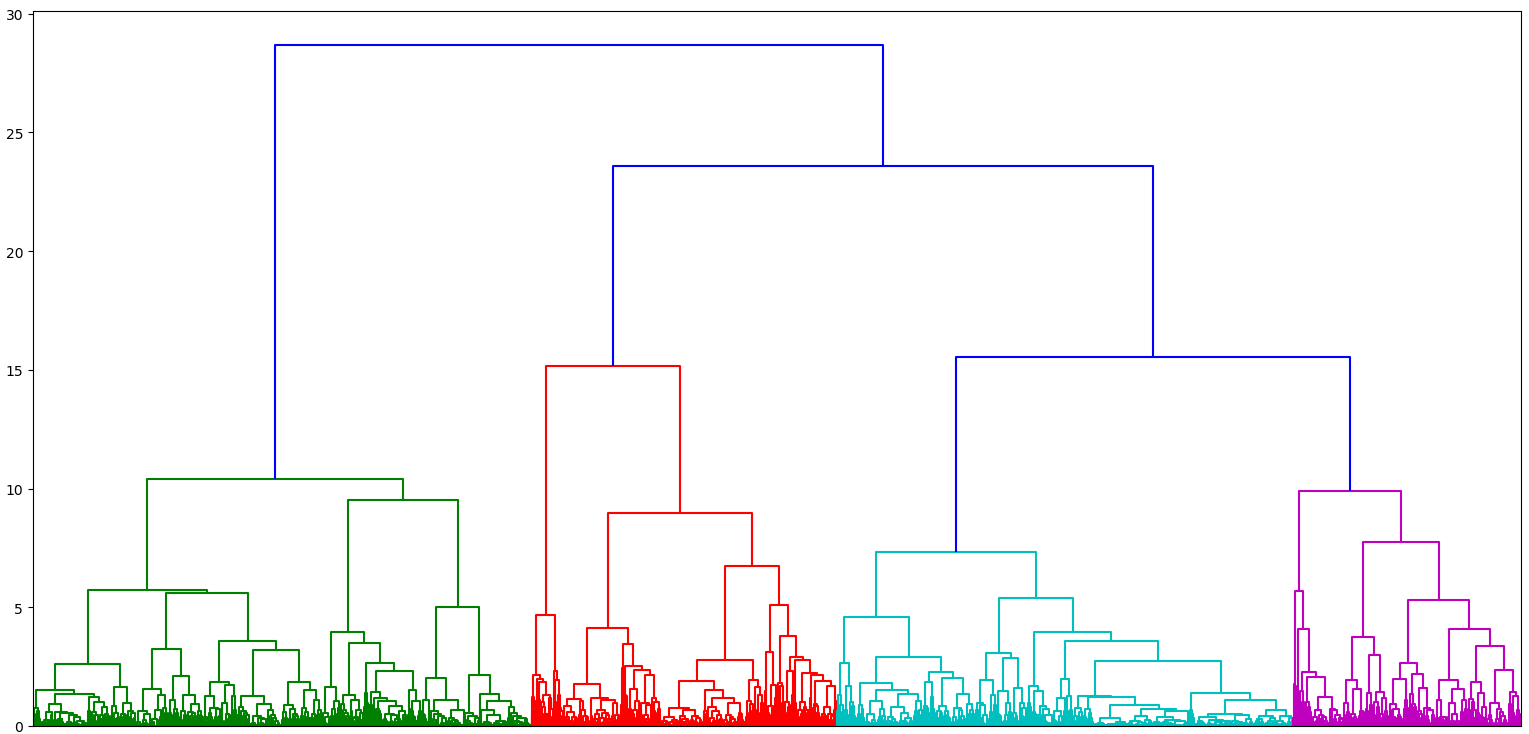
\includegraphics[width=\linewidth]{img/euclidean-ward.png}
  \caption{}\label{euward}
\endminipage\hfill
\minipage{0.48\textwidth}
  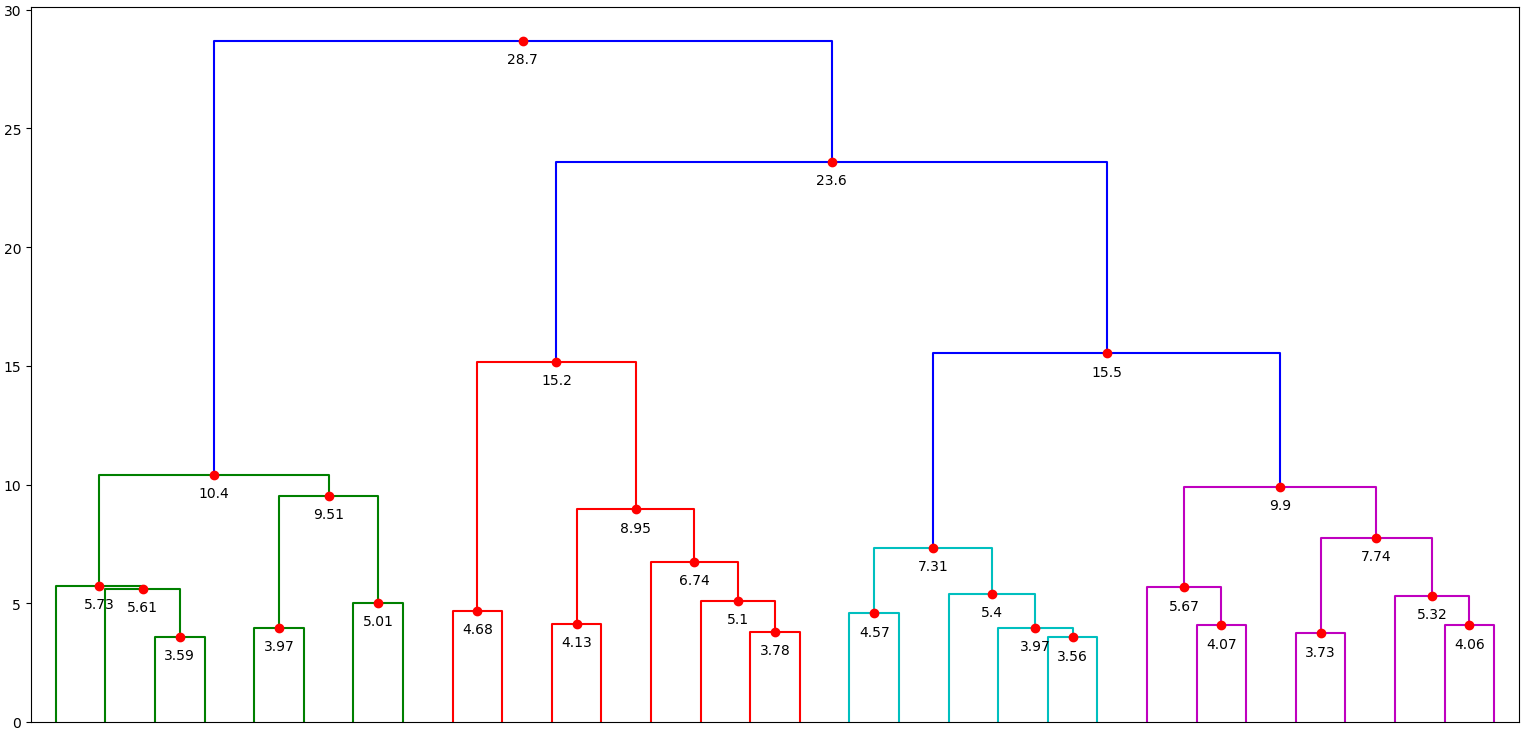
\includegraphics[width=\linewidth]{img/euclidean-ward-truncate.png}
  \caption{}\label{euwardtrunc}
\endminipage\hfill
\end{figure}

\begin{figure}[H]
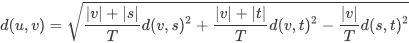
\includegraphics[width=0.5\linewidth]{img/ward_linkage.png}
\centering
\caption{Formula metodo di Ward}
\label{dendro-complete}
\end{figure} 

La Figura 2.7 descrive il metodo di Ward, metodo che cerca di minimizzare la varianza e generare cluster più coesi possibili. Nella formula $u$ è il cluster generato dai cluster $s$ e $t$, $v$ è un cluster inutilizzato e $T$ è la somma delle cardinalità dei cluster tale che $T = |v| + |s| + |t|$.

\newpage
I cluster ottenuti sono indicati da un numero per non confoderli in un primo momento con i cluster precedendentemente ottenuti. Dopo averli analizzati, di seguito vengono descritte le principali caratteristiche:
\paragraph{Cluster 1}
Composto da 2050 titolari di carta. Pagano in modo puntuale le alte spese che effettuano ogni mese. Non registrano ritardi e sono solito fare utilizzo del revolving credit per la rateizzazione. Rientrano tra i clienti credibili per la banca

\paragraph{Cluster 2}
Composto da 3353 titolari di carta. Compiono spese di bassa entità, pagandole in modo puntuale. Possono essere considerati i clienti meno a rischio per la banca.


\paragraph{Cluster 3}
Composto da 1530 persone. Registrano spese generalmente medio-alte con pagamenti generalmente bassi e registrando nella maggior parte dei casi ritardo nei pagamenti. Questo è il cluster che raggruppa i titolari di carta più a rischio con un alta percentuale di persone in credit\_default.


\paragraph{Cluster 4}
Composto da 3067 titolari di carta. Effettuano spese di media entità ma senza registrare ritardi nei pagamenti. Ogni mese pagano cifre discretamente basse, probabilmente ricorrendo all'utilizzo del revolving credit.
\mbox{}\\
\mbox{}\\
\begin{center}
\begin{tabular}{c|c|c|c|c|c|c}
	\hline
	\textbf{Cluster} & \textbf{ps-sep} 
	& \textbf{ps-aug} & \textbf{pa-sep} 
	& \textbf{pa-aug}\\
	\hline
	Cluster 1 & 
	$ -0.01 (\pm 0.5)$ & 
	$ -0.05 (\pm 0.46)$ &
	$11.8k (\pm 28.1k)$ &
	$14.2k (\pm 44.6)$\\
	\hline
	Cluster 2 & 
	$-0.68 (\pm 1.08)$ & 
	$-1.18 (\pm 0.72)$ &
	$4.8k (\pm 11.6k)$ &
	$4.8k (\pm 13.2k)$\\
	\hline
	Cluster 3 & 
	$1.7 (\pm 0.99)$ & 
	$1.8 (\pm 0.94)$ &
	$1.8k (\pm 3.3k)$ &
	$2.4k (\pm 3.9k)$\\
	\hline
	Cluster 4 & 
	$-0.10 (\pm 0.48)$ & 
	$-0.02 (\pm 0.56)$ &
	$4.2k (\pm 9.9k)$ &
	$3.4k (\pm 8.0k)$\\
	\hline
	& 
	\textbf{ba-sep} & 
	\textbf{ba-aug} & 
	\textbf{limit} & 
	\textbf{age} &\\
	\hline
	Cluster 1 & 
	$8.7k (\pm 21k)$ &
	$6.4k (\pm 16k)$ &
	$215k (\pm 126k)$ &
	$36 (\pm 8)$\\
	\hline
	Cluster 2 &
	$10.5k (\pm 21.8k)$ &
	$9k (\pm 19k)$ &
	$214.3k (\pm 125.3k)$ &
	$36 (\pm 8)$\\
	\hline
	Cluster 3 &
	$48.9k (\pm 49k)$ &
	$48k (\pm 48.1k)$ &
	$85.8k (\pm 71.7k)$ &
	$34 (\pm 9)$\\
	\hline
	Cluster 4 &
	$30.2k (\pm 24.3k)$ &
	$29.4k (\pm 22.7k)$ &
	$103.4k (\pm 85.4k)$ &
	$34 (\pm 9)$\\
	\hline
	& 
	\textbf{sex} & 
	\textbf{status} & 
	\textbf{education} & 
	\textbf{default}\\
	\hline
	Cluster 1 & 
	F &
	Single &
	University&
	12\%\\
	\hline
	Cluster 2 & 
	F &
	Single &
	Graduate School&
	15\%\\
	\hline
	Cluster 3 & 
	F &
	Single &
	University&
	60\%\\
	\hline
	Cluster 4 & 
	F &
	Single &
	University&
	16\%\\
	\hline
\end{tabular}
\end{center}

